\section{Kingman's Coalescent}
Consider a system of $L$ well mixed, coalescing particles. Each of the $\tbinom{L}{2}$ pairs of particles coalesces independently with rate $1$. This can be interpreted as generating an ancestral tree of $L$ individuals in a population model, tracing back to a single common ancestor.
\begin{enumerate}
    \item[(a)] Let $N_t$ be the number of particles at time $t$ with $N_0 = L$. Give the transition rates of the process $(N_t : t \ge 0)$ on the state space $\{1,\cdots,L\}$. Write down the generator $(\mathcal{L}f)(n)$ for $n \in \{1, \cdots,L\}$ and the master equation. Is the process ergodic? Does it have absorbing states? Give all stationary distributions. 
     
    \textit{ Sol. }  It's easy to see $G_{i,i-1} = \tbinom{i}{2} \times 1 = \tbinom{i}{2}$, for $i \in \{2, \cdots, L\}$. Since $\sum_{j=1}^L G_{i,j} = 0$ and $G_{i,j} = 0$ for $j \notin \{i-1, i\}$, we know $G_{i,i} = - \tbinom{i}{2}$. To summarize,
    \begin{equation}\label{eqn1}
    G_{i,j} = \begin{cases}
        \binom{i}{2} \qquad & j = i - 1, \, i \in \{2, \cdots, L\} \\ 
        -\binom{i}{2} \qquad & j = i, \, i \in \{2, \cdots, L\} \\ 
        0 \qquad & \text{Otherwise}
    \end{cases}.
    \end{equation}
    By $\mathcal{L}(f)(n) = \sum_{k \neq n} G_{n, k} [f(k) - f(n)]$ and \eqref{eqn1}, we know 
    \begin{equation}
        \mathcal{L}(f)(n) = \begin{cases}
            0 \qquad & n = 1 \\ 
            \binom{n}{2}[f(n-1) -f(n)] \qquad & n \in \{2,\cdots, L\}
        \end{cases}.
    \end{equation}
    The master equation is $\frac{\dif}{\dif t} \mbf{\pi}_t(x) = \sum_{y \neq x}\mbf{\pi}_t(y) G_{y,x} - \sum_{y \neq x} \mbf{\pi}_t (x) G_{x,y}$. Use \eqref{eqn1} again, and we get
    \begin{equation}
        \left\{ 
        \begin{array}{l}
            \frac{\dif \mbf{\pi}_t(1)}{\dif t} = \mbf{\pi}_t(2) \\ 
              \\ 
            \frac{\dif \mbf{\pi}_t(i)}{\dif t} = \binom{i+1}{2} \mbf{\pi}_t(i+1) - \binom{i}{2} \mbf{\pi}_t(i),\, i = 2,\cdots,L-1\\ 
             \\ 
            \frac{\dif \mbf{\pi}_t(L)}{\dif t} = -\binom{L}{2} \mbf{\pi}_L
        \end{array}
        \right. 
        .
    \end{equation}

    Obviously, state $1$ is absorbing, and furthermore, it forms an absorbing component $\{1\}$. Thus, the process is SP-ergodic.

    To find all stationary distributions, we need to solve $\mbf{\pi} G = \vec{0}$ with $\mbf{\pi}_t \in \Delta$, which is equivalent to 
    \begin{equation}\label{eqn2}
        \left\{ 
        \begin{array}{l}
            0 \mbf{\pi}_t(1) + \binom{2}{2} \mbf{\pi}_t(2) = 0\\ 
             \\ 
            - \binom{i}{2} \mbf{\pi}_t(i) + \binom{i+1}{2} \mbf{\pi}_t(i+1) = 0, \, i = 2, \cdots, L-1 \\ 
             \\ 
            - \binom{L}{2} \mbf{\pi}_t(L) = 0
        \end{array}
        \right. 
        .
    \end{equation}
    and 
    \begin{equation}\label{eqn3}
        \sum_{i=1}^L \mbf{\pi}_t(i) = 1.
    \end{equation}
    Using backward substitution performed on \eqref{eqn2} results in $\mbf{\pi}_t(i) = 0$, for $i = 2,\cdots, L$. And using \eqref{eqn3}, we have $\mbf{\pi}_t(1) = 1$. So the only stationary distribution is 
    \begin{equation*}
        \mbf{\pi}_t = [\ 1, \, \underbrace{0, \cdots,\, 0}_{(L-1)'s \,0}\ ].
    \end{equation*}
    \item[(b)] Show that the mean time to absorption is given by $\mbb{E}(T) = 2 \left( 1 - \frac{1}{L} \right)$. 
 
    \textit{ Sol. } Let $W_i$ be the holding time for the process to leave state $i$, i.e. $W_i = \inf \{t \in \mathbb{R}_+ | N_t \neq i,\, N_0 = i \}$, for $i = L, L-1, \cdots, 2$. Notice that
    \begin{equation}\label{eqn4}
        T = \sum_{i=2}^L W_i
    \end{equation}
    since the process can only go from state $i$ to $i-1$ at a time.
    
    From lecture, we know $W_i \sim \text{Exponential}(|G_{i,i}|)$. So 
    \begin{equation}\label{eqn5}
        \mathbb{E}[W_i] = \frac{1}{|G_{i,i}|} = \frac{1}{\binom{i}{2}} = \frac{(i-2)! \times 2!}{i!} = \frac{2}{i(i-1)}.
    \end{equation}
    Thus, using \eqref{eqn4} together with the linearity of expectation and \eqref{eqn5}, we get 
    \begin{align*}
        \mathbb{E}(T) = & \mathbb{E} \left(\sum_{i = 2}^L W_i \right) \\ 
        = & \sum_{i = 2}^L  \mathbb{E}(W_i) \\ 
        = & \sum_{i = 2}^L \left( \frac{2}{i(i-1)} \right) \\ 
        = & \sum_{i = 2}^L 2 \left( \frac{1}{i-1} - \frac{1}{i} \right) \\ 
        = & 2 \left(1 - \frac{1}{L} \right).
    \end{align*}

    \item[(c)] Write the generator of the rescaled process $(N_t/L: t \ge 0)$ and Taylor expand it up to the second order. Show that the slowed-down, rescaled process $(X^L_t: t\ge 0)$ where 
    $$X^L_t := \frac{1}{L}N_{\frac{t}{L}},$$
    converges to the process $(X_t: t \ge 0)$ with generator 
    $$\bar{\mathcal{L}}f(x) = - \frac{x^2}{2} f'(x)$$
    and state space $(0, 1]$ with $X_0 = 1$.
    
    Convince yourself that this process is ``deterministic'', i.e. $X_t = \mathbb{E}(X_t)$ for all $t \ge 0$, and compute $X_t$ explicitly. How is your result compatible with the result from (b)?

    \textit{ Sol. } For the rescaled process $(N_t / L: t \ge 0)$, the rates of transitions are not changed, but the state space is replaced with $\{\frac{1}{L}, \cdots, \frac{L}{L}\}$. Thus, the rate matrix is 
    \begin{equation}\label{eqn6}
        G_{i,j} = \begin{cases}
            \binom{iL}{2} \qquad & j = i - \frac{1}{L}, \, i \in \{\frac{2}{L}, \cdots, \frac{L}{L}\} \\ 
            -\binom{iL}{2} \qquad & j = i, \, i \in \{\frac{2}{L}, \cdots, \frac{L}{L}\} \\ 
            0 \qquad & \text{Otherwise}
        \end{cases}
    \end{equation}
    By $(\mathcal{L}f)(n) = \sum_{k \neq n} G_{n,k} [f(k) - f(n)]$ and \eqref{eqn6}, we have 
    \begin{equation}\label{eqn7}
        \mathcal{L}(f)(n) = 
        \begin{cases}
            0 \qquad & n = \frac{1}{L} \\ 
            \binom{nL}{2} [f(n-\frac{1}{L}) - f(n)] \qquad & n \in \{\frac{2}{L}, \cdots, \frac{L}{L}\}
        \end{cases}.
    \end{equation}
    Now Taylor expand \eqref{eqn7} to the sencond order, which results in 
    \begin{equation*}
        \mathcal{L}(f)(n) = 
        \begin{cases}
            0 \qquad & n = \frac{1}{L} \\ 
            \binom{nL}{2} [-\frac{1}{L} f'(n) + \frac{1}{2L^2}f''(n) + o(\frac{1}{L^2})] \qquad & n \in \{\frac{2}{L}, \cdots, \frac{L}{L}\}
        \end{cases}.
    \end{equation*}

    We need to derive the generator of the process $(X_t^L: t \ge 0)$ first. The rate matrix of $(X_t^L: t\ge 0 )$ is 
    \begin{equation}\label{eqn8}
        G_{i,j} = \begin{cases}
            \frac{1}{L}\binom{iL}{2} \qquad & j = i - \frac{1}{L}, \, i \in \{\frac{2}{L}, \cdots, \frac{L}{L}\} \\ 
            -\frac{1}{L}\binom{iL}{2} \qquad & j = i, \, i \in \{\frac{2}{L}, \cdots, \frac{L}{L}\} \\ 
            0 \qquad & \text{Otherwise}
        \end{cases}.
    \end{equation}

    By $(\mathcal{L}f)(n) = \sum_{k \neq n} G_{n,k} [f(k) - f(n)]$ and \eqref{eqn8}, we have 
    \begin{equation}\label{eqn9}
        \mathcal{L}(f)(n) = 
        \begin{cases}
            0 \qquad & n = \frac{1}{L} \\ 
            \frac{1}{L}\binom{nL}{2} [f(n-\frac{1}{L}) - f(n)] \qquad & n \in \{\frac{2}{L}, \cdots, \frac{L}{L}\}
        \end{cases}.
    \end{equation}

    Notice that 
    \begin{eqnarray*}
        \lefteqn{\frac{1}{L} \binom{nL}{2} \left[ f(n - \frac{1}{L}) - f(n)\right]} \\ 
        &=& \frac{1}{L} \cdot \frac{(nL)!}{(nL-2)!2!} \cdot \left[ f(n) - \frac{1}{L} f'(n) + \frac{1}{2L^2} f''(n) + o(\frac{1}{L^2}) - f(n) \right] \\ 
        &=& \frac{1}{L} \cdot \frac{(nL)(nL-1)}{2} \cdot \left[ -\frac{1}{L} f'(n) + \frac{1}{2L^2} f''(n) + o(\frac{1}{L^2}) \right] \\ 
        &=& \frac{n(nL-1)}{2} \cdot \left[ -\frac{1}{L} f'(n) + \frac{1}{2L^2} f''(n) + o(\frac{1}{L^2})\right] \\ 
        &=& \frac{n}{2}\left[ -\frac{nL-1}{L}f'(n) + \frac{nL-1}{2L^2}f''(n) + o(\frac{nL-1}{L^2})\right],
    \end{eqnarray*}
    so as $L \to \infty$, we have 
    $$\lim_{L \to \infty} \frac{1}{L} \binom{nL}{2} \left[ f(n - \frac{1}{L}) - f(n) \right] = - \frac{n^2}{2} f'(n).$$
    In conclusion, we have, as $L \to \infty$, the process $(X_t^L: t \ge 0)$ converges to $(X_t: t \ge 0)$ with generator 
    \begin{equation} \label{eqn10}
        \bar{\mathcal{L}}(f)(x) = - \frac{x^2}{2} f'(x)
    \end{equation}
    and state space $(0, 1]$ with $X_0 = 1$.
    
    \item[(d)] Generate sample paths of the process $(X_t^L: t \ge 0)$ for $L = 10$, $L = 100$, $L = 1000$ and compare to the solution $X_t$ from (c) in a single plot.
      
    \textit{ Sol. }
    \lstinputlisting[language=Python]{problem1d.py}
    The output image is Figure \ref{fig1}.
    \begin{figure}[h!]
        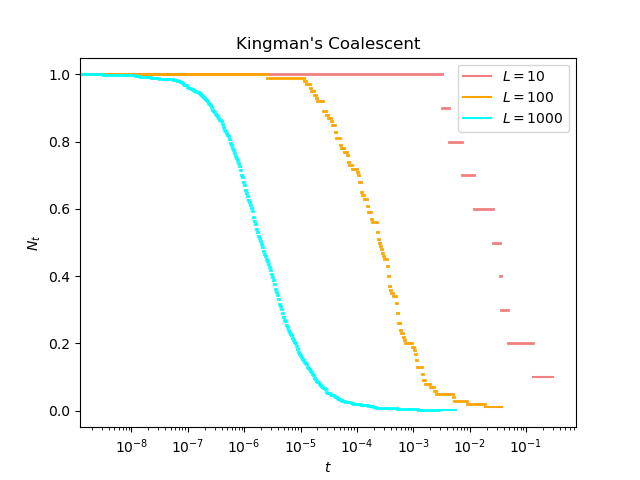
\includegraphics[width=18cm]{Kingman_Coalescent.png}
        \caption{Kingman's Coalescent with $L = 10$, $L = 100$, $L = 1000$}
        \label{fig1}
    \end{figure}
\end{enumerate}